% AIAA3201 Project 2 report -- CVPR two-column layout (official author-kit style files)
% Compile: tectonic main.tex   (or pdflatex + bibtex + pdflatex x2 on Overleaf)
% Review option keeps page numbers; switch to \usepackage{cvpr} for a camera-ready look.

\documentclass[10pt,twocolumn,letterpaper]{article}
\usepackage[pagenumbers]{cvpr}
% Packages beyond the CVPR style file, loaded before hyperref (see main.tex).
\usepackage{booktabs}        % already pulled in by cvpr.sty; kept explicit for clarity
\usepackage{multirow}
\usepackage{graphicx}

% ---- visible TODO marker: every \tbd must be resolved before submission (see README)
\newcommand{\tbd}[1]{\textcolor{red}{[TBD: #1]}}
% reference to a figure/table/section that B's part will introduce
\newcommand{\bsec}[1]{\textcolor{red}{(#1 -- B's branch)}}

% compact numbers in tables
\newcommand{\best}[1]{\textbf{#1}}
\newcommand{\std}[1]{{\scriptsize$\pm$#1}}

\setlength{\tabcolsep}{3.2pt}


\definecolor{cvprblue}{rgb}{0.21,0.49,0.74}
\usepackage[pagebackref=false,breaklinks,colorlinks,allcolors=cvprblue]{hyperref}

%%%%%%%%% TITLE
\title{How Far Can a Frozen Encoder Carry Few-Shot Industrial Anomaly Detection?\\
A Controlled Study on VisA}

%%%%%%%%% AUTHORS
\author{Sibei Lyu\thanks{Equal split of work is documented in the project repository:
visual branch, protocol and analysis by S.L.; multimodal branch, demo and packaging by
the co-author. Code and every number in this report are reproducible from
\texttt{github.com/BEBE2777/computer-vision-aiaa3201}.}\\
The Hong Kong University of Science and Technology (Guangzhou)
\and
Co-author (multimodal branch)\tbd{B's name}\\
The Hong Kong University of Science and Technology (Guangzhou)}

\def\confName{AIAA3201}
\def\confYear{2026}

\begin{document}
\maketitle

\begin{abstract}
Few-shot industrial anomaly detection asks a frozen representation, learned elsewhere and
once, to decide whether a new image of a product deviates from a handful of defect-free
references. We reproduce the strongest training-free visual recipe, AnomalyDINO, on the six
object-centric categories of VisA under its official configuration (94.61 image AUROC at
1-shot, rising to 96.62 at 8-shot), then hold the scoring pipeline fixed and change exactly
one variable at a time. Replacing the self-supervised DINOv2 encoder with CLIP's vision tower
costs 5.6 image-AUROC points at 1-shot and the deficit does not close with more references;
patch-level measurements attribute it to strongly anisotropic CLIP features whose distance
maps leave normal background variance close to the decision threshold. An image-level
crossing of the two arms' verdicts shows they agree on only 63.2\% of the 960 test images and
that CLIP is right on 58 images where DINOv2 is wrong -- countable complementarity that a
pre-registered, calibration-based score-level fusion exploits: at the pre-registered weight
the fused score gains $+0.68$ points over the better single arm, averaged over nine
(shot, seed) cells, and cuts the spread across cells from 0.88 to 0.59 points. A frozen
multimodal branch (Qwen2-VL-7B, forced-choice scoring) obtains 95.75 macro image AUROC
on 696 images held out from its pilots (DINOv2: 93.13; CLIP: 85.30, 1-shot seed~0)
and correctly classifies 48 of the 73 images both visual arms miss at their calibrated thresholds; its equal-weight fusion with DINOv2 is reported as a post-hoc
exploration only. We further report an honest reliability accounting:
thresholds calibrated on 20 normal images realise false-alarm rates of 9.4--21.4\% at a
nominal 5\%, so operating points are reported as achieved, not assumed. Code, per-image
scores and every number in this report are available at
\url{github.com/BEBE2777/computer-vision-aiaa3201}.
\end{abstract}

\section{Introduction}
\label{sec:intro}

Industrial visual inspection asks a narrow question under unforgiving constraints: given a
handful of defect-free images of one product, decide whether a new image contains a defect,
and where. Collecting defective samples of a rare failure mode is expensive by definition,
and a line re-tooled for a new product cannot wait for a labelled corpus. Few-shot anomaly
detection therefore inverts the usual recipe: instead of fitting a model to many labelled
examples of a fixed task, it asks how far a \emph{frozen} representation, learned elsewhere
and once, can be pressed into service for a product it has never seen.

Two families of answers exist. The first stays purely visual: model normal appearance from
the few references and flag deviations from it, a line running from handcrafted template
comparison through statistical patch models to self-supervised
features~\cite{bergmann2019mvtec,defard2021padim,roth2022patchcore,oquab2024dinov2,damm2025anomalydino}.
The second brings language in: vision--language models let an inspector describe
``defect-free'' in words and transfer it across
products~\cite{radford2021clip,jeong2023winclip,zhou2024anomalyclip}. Between them lies an
open empirical question -- which kind of frozen evidence separates a subtle scratch from a
shift in pose or lighting -- and a systems question of whether the two can be combined into
something better than either alone.

This report treats that junction as a controlled measurement. Part~2 reproduces
AnomalyDINO~\cite{damm2025anomalydino} on the six object-centric categories of
VisA~\cite{zou2022spot} and verifies it cell-by-cell against the official pipeline. Part~3
changes one variable at a time: (\textbf{E1}) the visual encoder, swapping DINOv2 for CLIP's
vision tower under an identical scoring rule; (\textbf{E2}) a multimodal inspector (Qwen-VL)
that sees the references and the test image; and calibrated score-level fusion of the
branches. Visual fusion was specified in advance. Qwen's score direction was selected on
a pilot and fixed for holdout scoring; Qwen fusion was exploratory.

Our contributions are:
\begin{itemize}
  \item a verified AnomalyDINO reproduction on VisA (all 72 protocol cells agree with the
        official pipeline to the last printed digit), plus the two harness defects found and
        fixed on the way (cache-key collisions, a float16 feature cache);
  \item a controlled encoder swap showing that language alignment costs 5.6 image-AUROC
        points at 1-shot, does not close with more references, and reverses on one category
        -- with the mechanism measured at the patch level (feature anisotropy), not asserted;
  \item an image-level error taxonomy (63.2\% verdict agreement; 58 images only CLIP solves)
        and a pre-registered fusion that gains $+0.68$ points over the better arm across
        nine (shot, seed) cells while exposing a calibration gap (nominal 5\%, realised
        9.4--21.4\%);
  \item a frozen multimodal branch (Qwen2-VL-7B, forced-choice scoring) evaluated on the 696
        test images held out from its own development pilots, with the highest macro AUROC point estimate
        (95.75 vs.\ 93.13 DINOv2 / 85.30 CLIP macro AUROC) and right on 48 of the 73 images
        both visual arms miss -- with its fusion with DINOv2 reported strictly as post-hoc.
\end{itemize}

\section{Related Work}
\label{sec:related}

\paragraph{Industrial anomaly detection and its benchmarks.}
Industrial inspection is usually cast as normal-only learning: the training set contains
defect-free images, and a defect is any deviation from the modelled normal
appearance~\cite{bergmann2019mvtec}. MVTec AD~\cite{bergmann2019mvtec} established the
evaluation protocol of image-level detection plus pixel-level localisation, and later work
extended it to larger and more varied data: VisA~\cite{zou2022spot} offers ten product
categories with subtle, low-contrast defects (we use its six object-centric categories), and
MVTec AD~2~\cite{hecklerkram2026mvtec2} adds transparent objects and severe lighting
variation to expose the remaining headroom of current methods. Our protocol follows this
line, including the separation of image AUROC (the primary metric) from pixel AUROC, and the
use of a held-out set of normal images for score calibration rather than for model fitting.

\paragraph{Nearest-neighbour and statistical modelling of patch features.}
A first family of methods compares each test location against a model of normal appearance
built from pretrained features. SPADE~\cite{cohen2021spade} scores a test image by the
distance to its nearest neighbours in the training set, with a pixel-level variant that
aligns intermediate activations; PaDiM~\cite{defard2021padim} models the per-patch feature
distribution as a multivariate Gaussian and scores by Mahalanobis distance;
PatchCore~\cite{roth2022patchcore} refines the nearest-neighbour recipe with a
coreset-subsampled memory bank and reports near-saturated full-shot results on MVTec AD. All
three inherit the inductive bias our Part~2 baseline uses -- a \emph{frozen} general feature
extractor plus a normality model that never sees a defect -- and differ mainly in what
``normal'' is modelled as and how much memory it needs.

\paragraph{Reconstruction and synthesis.}
A second family learns to reconstruct or synthesise normal appearance and flags what
reconstruction fails to explain. CutPaste~\cite{li2021cutpaste} trains a classifier on
self-generated, unnatural perturbations; DRAEM~\cite{zavrtanik2021draem} pairs a
reconstruction network with a discriminative head on simulated defects. These methods are
effective but need a large training corpus of the very product under inspection, which is the
regime few-shot inspection explicitly excludes; we therefore do not compare against them
numerically, but they motivate the synthetic-defect direction we keep as a possible
calibration aid rather than a scoring rule.

\paragraph{Foundation-model features and few-shot inspection.}
The decisive change for the few-shot regime is representation quality rather than the
normality model. DINOv2~\cite{oquab2024dinov2} produces dense, locally discriminative patch
features from self-supervised pretraining, and AnomalyDINO~\cite{damm2025anomalydino} shows
that simply running patch-level nearest neighbours on those features -- training-free, no
fine-tuning, no auxiliary data -- rivals and often exceeds vision--language few-shot methods.
RegAD~\cite{huang2022regad} instead \emph{trains} a category-agnostic registration model
across many categories so that new categories need no re-training; it demonstrates that
few-shot methods can share structure across products, at the cost of a training phase our
setting does not allow. On the systems side, EfficientAD~\cite{batzner2024efficientad} shows
that millisecond-level inference is compatible with high accuracy, which frames the cost
accounting we report for our own runs. Our Part~2 is the official AnomalyDINO recipe; our
Part~3 asks whether its conclusion -- \emph{good frozen visual features are enough} --
survives a change of the frozen encoder, which AnomalyDINO itself does not test.

\paragraph{Language-aligned encoders, used vision-only.}
CLIP~\cite{radford2021clip} aligns images with text and dominates zero-/few-shot transfer
through prompts: WinCLIP~\cite{jeong2023winclip} aggregates window- and patch-level features
against handcrafted normal/abnormal state words, and
AnomalyCLIP~\cite{zhou2024anomalyclip} learns object-agnostic prompts so that one text prompt
transfers across product categories. Both operate on the \emph{text} side of the alignment;
the dense quality of CLIP's \emph{vision tower} -- what its patch tokens say before any
prompt is applied -- is rarely examined. Our E1 fills exactly that gap: we take patch tokens
from the CLIP vision encoder, keep the $k$-NN scoring rule, resolution, reference sampling
and calibration identical to the DINOv2 control, and measure how much language alignment
costs dense anomaly matching.

\paragraph{Reliability of the decision, not just the score.}
Anomaly scores are only useful through a threshold, and thresholds inherit the failure modes
of probability calibration~\cite{guo2017calibration}. Following the risk--coverage view of
selective prediction~\cite{geifman2017selective}, we derive every OK/NG threshold from 20
held-out normal calibration images and report the achieved false-alarm rate rather than
assuming the nominal 5\%. Segmentation prompts such as SAM~\cite{kirillov2023sam} offer a
complementary route to background suppression that we discuss as future work rather than use,
because a mask from a general segmenter would add a second moving part to a comparison
designed to keep the backbone the only variable.

\paragraph{Positioning.}
Existing work either trains on the target product
\cite{li2021cutpaste,zavrtanik2021draem,huang2022regad}, freezes one vision backbone
\cite{damm2025anomalydino,roth2022patchcore}, or moves the comparison to the text side of a
vision--language model~\cite{jeong2023winclip,zhou2024anomalyclip}. What is missing is a
controlled measurement of \emph{which frozen encoder} dense nearest-neighbour matching should
run on, and an error analysis that says where the encoders disagree rather than only how far
apart their averages are. The complementary question -- whether a multimodal model asked
directly, in language, about reference and test images adds information that neither
encoder's score contains -- is reviewed in \bsec{the vision--language subsection of Related
Work}.

\section{Method}
\label{sec:method}

\subsection{Task, data and protocol}
\label{sec:method-protocol}

We evaluate on six categories of VisA (candle, capsules, cashew, chewinggum, fryum,
pipe\_fryum) in the few-shot setting, with 1, 2, 4 and 8 normal reference images per category
and three sampling seeds (0/1/2). For every category the first 20 training images are held
out as a \emph{calibration set} and never used as references; the remaining normal images
form the pool from which the $k$-th shot of the $s$-th seed is drawn
($\text{pool}[s \cdot \text{shot} : (s{+}1) \cdot \text{shot}]$), so every method sees
exactly the same references for a given (shot, seed). The same 960 test images are scored by
every system.

Two metrics are reported. Image-level AUROC uses the mean of the top 1\% of the pixel
distance map as the anomaly score, as in AnomalyDINO~\cite{damm2025anomalydino}. Pixel-level
AUROC is computed on maps resampled to $448\times448$ for all methods, because pooling the
native-resolution pixels of all images does not fit in the shared GPU memory; the same
resampling is applied everywhere, so comparisons stay well defined. Mean\,$\pm$\,std is always
taken over seeds: the six-category mean is formed per seed first, and the standard deviation
is taken over the three per-seed means. The decision threshold, used only for the
qualitative error analysis and the OK/NG operating points, is the 95th percentile of the
scores of the 20 calibration images -- it never sees a test label.
Figure~\ref{fig:pipeline} summarises the full pipeline.

\begin{figure*}[t]
  \centering
  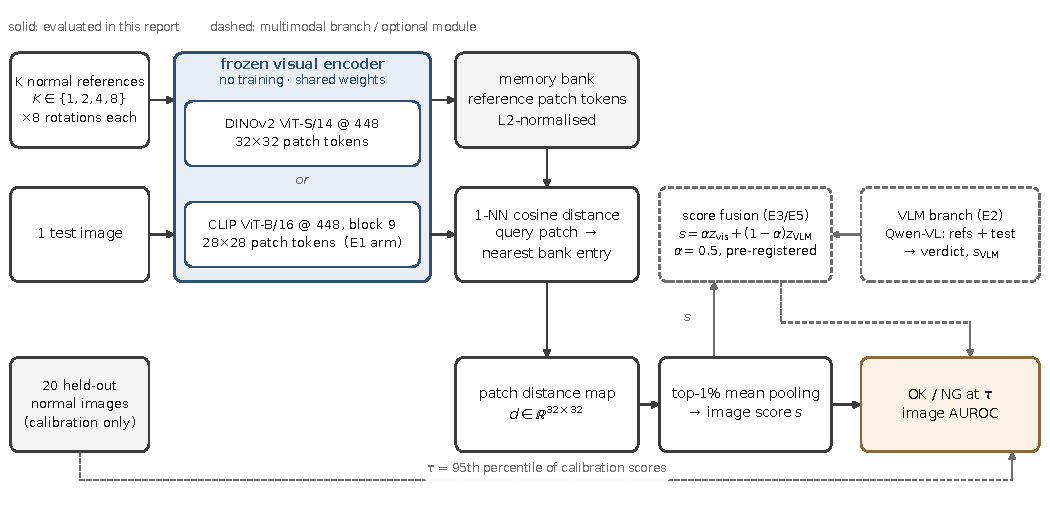
\includegraphics[width=\textwidth]{figures/pipeline.pdf}
  \caption{Overview of the pipeline under the frozen protocol. The support path builds an
  L2-normalised memory bank from $K$ normal references and their 8 rotations; the query path
  pushes the test image through the \emph{same} frozen encoder, scores every patch by 1-NN
  cosine distance against the bank, and pools the top 1\% of the distance map into the image
  score. The two encoders are interchangeable arms (E1) that share everything else. The
  dashed modules are optional: score-level fusion with the multimodal branch (E2--E5), and
  the decision threshold, which is derived from 20 held-out normal calibration images only.}
  \label{fig:pipeline}
\end{figure*}

\subsection{Part 1 -- template-difference baseline}
\label{sec:method-part1}

The baseline treats the reference set as a template. Images are resized so that the shorter
edge is 448 and centre-cropped, because a pixel-wise comparison needs a common frame; ECC
registration maps every image onto the first reference; the difference between a test image
and a reference is $0.5\,|\Delta I| + 0.5\,(1 - \mathrm{SSIM})$; the closest template (lowest
mean difference) becomes the anomaly map, which is Gaussian-smoothed and aggregated with the
same top-1\% mean as AnomalyDINO so that image AUROC stays comparable. Scores are never
rescaled per image. The baseline needs no training and no pretrained weights, and it fixes
the lower bound of the comparison: a pretrained-feature method that does not beat it is not
earning its complexity.

\subsection{Part 2 -- verified AnomalyDINO reproduction}
\label{sec:method-part2}

AnomalyDINO extracts dense patch features from DINOv2 ViT-S/14 at 448 ($32\times32$ patch
grid), builds a memory bank from the reference patches (each reference contributes eight
rotations, which makes the bank rotation-tolerant), and scores a test patch by its L2
distance to the nearest bank entry; the pixel map is the upsampled distance field, smoothed
with a Gaussian. We first reproduced this pipeline with the official code, then
re-implemented the scoring in a cached runner so that Part~3 variants can be compared without
re-extracting features.

The re-implementation is verified rather than assumed: a parity probe compares the two
pipelines cell by cell, and after the fixes described below all 72 cells (6 categories
$\times$ 4 shots $\times$ 3 seeds) agree with the official run to the last printed digit. Two
defects were found and fixed on the way, and both matter for Part~3:
\begin{enumerate}
  \item \textbf{Cache-key collision.} VisA reuses file names across splits (capsules shares
        eight basenames between \texttt{test/good} and \texttt{test/bad}, and ${\sim}90$
        between \texttt{train/good} and \texttt{test/bad}). A basename-keyed feature cache
        therefore served a defective image the features of a normal image with the same name,
        which cost up to 5 image-AUROC points on capsules. Cache keys are now namespaced by
        the parent directory.
  \item \textbf{Lossy cache dtype.} Storing cached features as float16 perturbed query
        features by up to ${\sim}8\times10^{-3}$, enough to change the top-1\% nearest
        neighbours of borderline images; the cache is now float32.
\end{enumerate}

\subsection{E1 -- replacing the backbone with CLIP}
\label{sec:method-e1}

The question E1 asks is narrow: with the scoring rule, the reference sampling, the
calibration and the resolution all held fixed, what changes when the dense features come from
a language-aligned image encoder (CLIP ViT-B/16) instead of a self-supervised one (DINOv2
ViT-S/14)? DINOv2 features are trained to be locally discriminative, which is what a
nearest-neighbour patch matcher wants; CLIP features are trained to place a whole image next
to a text description, and are known to be strongly anisotropic at the patch level. Whether
that costs accuracy in few-shot anomaly detection is an empirical question.

\paragraph{Extracting patch tokens from CLIP.}
\texttt{clip.encode\_image} returns only the pooled global feature, so the patch tokens are
taken from the vision tower directly: the input is patch-embedded, passed through the
transformer blocks, and for block $l$ we take the residual-stream output, drop the class
token, apply \texttt{ln\_post} and the projection matrix \texttt{proj} (so the vectors live
in the same space as the global embedding), and keep the remaining $g_h \times g_w$ tokens in
raster order. Three properties were verified explicitly, because a silent mistake in any of
them produces plausible-looking but wrong AUROC:
\begin{itemize}
  \item \textbf{Grid order.} A synthetic probe replaces one patch of the input with a white
        square; the argmax of the extracted tokens must be $\mathrm{row}\cdot14+\mathrm{col}$.
        It is ($5{\cdot}14{+}8 = 78$), confirming raster order.
  \item \textbf{Positional embedding at 448.} CLIP is trained at 224 with a $14{\times}14$
        position grid; a 448 input produces a $28{\times}28$ grid, so the learned position
        table is interpolated bicubically to the actual (rectangular) grid shape. An occlusion
        probe checks that the score map responds at the occluded location: the argmax lands
        within 3 patches of the true occlusion centre.
  \item \textbf{Forward equivalence.} For the native 224 input, our manual forward and the
        official \texttt{encode\_image} agree bit-for-bit on the class token, so the token
        extraction path introduces no off-by-one block or missing normalisation.
\end{itemize}
The resulting wrapper mirrors the DINOv2 interface
(\texttt{prepare\_image} $\rightarrow$ \texttt{extract\_layers}), which lets the same cached
scoring pipeline evaluate both backbones; no scoring code is duplicated.

\paragraph{Choices frozen before the grid.}
A pilot (candle and capsules, 1-shot, seed 0) fixed four settings; none were tuned on the
test split afterwards.
\begin{itemize}
  \item \textbf{Resolution 448, not 224.} The interpolated position table is stable at 448,
        so we keep the same resolution as Part~2 instead of falling back to CLIP's native
        224; the control is DINOv2 at 448.
  \item \textbf{Layer 9 of 12.} Patch features were swept over blocks 6, 9 and 12. The last
        block is the most anisotropic in CLIP (mean pairwise cosine similarity of patch
        features inside one image 0.57--0.67, against 0.36 for DINOv2 L12) and its dense
        matching suffers for it: at 1-shot on the pilot, block 12 scored 69.4 image AUROC on
        candle against 89.9 for block 9 under the same framing. Block 9 has the lowest
        anisotropy of the three and the best pixel AUROC under the frozen framing; blocks 6
        and 12 are reported as a sensitivity check, not as candidates.
  \item \textbf{No foreground mask, for both backbones.} AnomalyDINO's agnostic
        preprocessing estimates a foreground mask by PCA on DINOv2 features; the threshold is
        tied to that feature geometry and has no counterpart for CLIP. Rather than give one
        backbone a preprocessing advantage, E1 disables the mask for both, so the only
        difference between the two lines is the encoder.
  \item \textbf{\texttt{short\_edge} framing.} The official CLIP preprocessing centre-crops
        to a square, which cuts objects out of frame on categories whose objects are
        off-centre (capsules pixel AUROC dropped to 75.5 under the crop). \texttt{short\_edge}
        keeps the full frame and lets the patch grid be rectangular, matching the DINOv2
        wrapper; the same framing is used for both backbones.
\end{itemize}

\subsection{Fusion protocol and the multimodal branch}
\label{sec:method-fusion}

Fusion is pre-registered before any outcome is seen: each branch's score is standardised per
category with the median and MAD of its scores on the 20 held-out normal calibration images
(falling back to the standard deviation, then to a constant, when the MAD degenerates), and
the fused score is $\alpha z_1 + (1-\alpha) z_2$ with the main result at $\alpha = 0.5$; the
five-point $\alpha$ sweep is reported as a sensitivity analysis, never as a tuned optimum, and
no test label participates in any choice~\cite{guo2017calibration}. The machinery is checked
with a consistency requirement: $\alpha{=}1$ and $\alpha{=}0$ must reproduce the single
branches exactly. \bsec{E2: Qwen-VL branch description, prompts, decoding and per-image
scores} completes the taxonomy's fourth cell and feeds E3--E5.

\section{Experiments}
\label{sec:experiments}

\subsection{Setup}
\label{sec:exp-setup}

Four systems are compared on the protocol of \S\ref{sec:method-protocol}.
\textbf{Part~1} is the template-difference baseline (\S\ref{sec:method-part1}).
\textbf{Part~2} is the official AnomalyDINO reproduction (DINOv2 ViT-S/14 @448, agnostic
preprocessing, PCA foreground mask), verified cell-by-cell against the published pipeline.
\textbf{E1 control} is DINOv2 @448 with the mask disabled -- the identical-scoring
counterpart of our CLIP arm. \textbf{E1 CLIP} is CLIP ViT-B/16 @448, block 9,
\texttt{short\_edge} framing, no mask, with patch tokens extracted and probe-verified as
described in \S\ref{sec:method-e1}. The controlled pair (control vs CLIP) differs \emph{only}
in the encoder; Part~2 differs additionally in preprocessing -- its mask is worth
${\approx}1.3$ image points, measured as official minus control -- and is the complete-system
reference, not a controlled arm.

\subsection{Main results}
\label{sec:exp-main}

\begin{table}[t]
\centering
\caption{Image-level AUROC (\%), mean\,$\pm$\,std over three seeds of the six-category
means. The controlled pair is DINOv2-control vs CLIP; Part~2 adds the official PCA mask and
is a complete-system reference. Best per column in bold.}
\label{tab:image}
\footnotesize
\setlength{\tabcolsep}{2.2pt}
\begin{tabular}{lcccc}
\toprule
Method & 1-shot & 2-shot & 4-shot & 8-shot \\
\midrule
Template diff.\ (Part 1) & 52.00\,\std{1.13} & 54.08\,\std{3.38} & 55.36\,\std{3.22} & 57.96\,\std{0.47} \\
AnomalyDINO (Part 2, masked) & \best{94.61}\,\std{0.84} & \best{95.33}\,\std{0.46} & \best{96.15}\,\std{0.40} & \best{96.62}\,\std{0.57} \\
DINOv2 @448 nomask (ctrl) & 93.34\,\std{0.72} & 94.16\,\std{0.27} & 94.92\,\std{0.49} & 95.37\,\std{0.72} \\
CLIP @448 L9 nomask (E1) & 87.70\,\std{1.24} & 89.22\,\std{0.29} & 89.27\,\std{0.38} & 89.48\,\std{0.23} \\
\bottomrule
\end{tabular}
\end{table}

\begin{table}[t]
\centering
\caption{Pixel-level AUROC (\%), same aggregation as Table~\ref{tab:image}.}
\label{tab:pixel}
\footnotesize
\setlength{\tabcolsep}{2.2pt}
\begin{tabular}{lcccc}
\toprule
Method & 1-shot & 2-shot & 4-shot & 8-shot \\
\midrule
Template diff.\ (Part 1) & 65.06\,\std{0.41} & 64.85\,\std{0.39} & 65.47\,\std{0.29} & 66.14\,\std{0.22} \\
AnomalyDINO (Part 2, masked) & \best{98.08}\,\std{0.05} & \best{98.22}\,\std{0.07} & \best{98.36}\,\std{0.03} & \best{98.47}\,\std{0.01} \\
DINOv2 @448 nomask (ctrl) & 97.06\,\std{0.32} & 97.57\,\std{0.11} & 97.91\,\std{0.06} & 98.16\,\std{0.04} \\
CLIP @448 L9 nomask (E1) & 94.44\,\std{0.10} & 94.97\,\std{0.09} & 95.22\,\std{0.06} & 95.46\,\std{0.05} \\
\bottomrule
\end{tabular}
\end{table}

Under the controlled protocol, replacing DINOv2 with CLIP costs \textbf{5.6 image points at
1-shot} (87.70 vs 93.34) and 2.6 pixel points, and the deficit \textbf{does not close with
more references}: CLIP gains $+1.8$ image points from 1-shot to 8-shot, the DINOv2 control
gains $+2.0$, and the ordering never flips (Tables~\ref{tab:image},~\ref{tab:pixel};
Fig.~\ref{fig:shots}). The few-shot deficit is therefore a property of the features, not of
sample size. The official masked baseline sits another ${\approx}1.3$ image points above the
unmasked control at every shot count, which prices the PCA foreground mask and explains why
it was removed from both controlled arms rather than granted to one.

\begin{figure}[t]
  \centering
  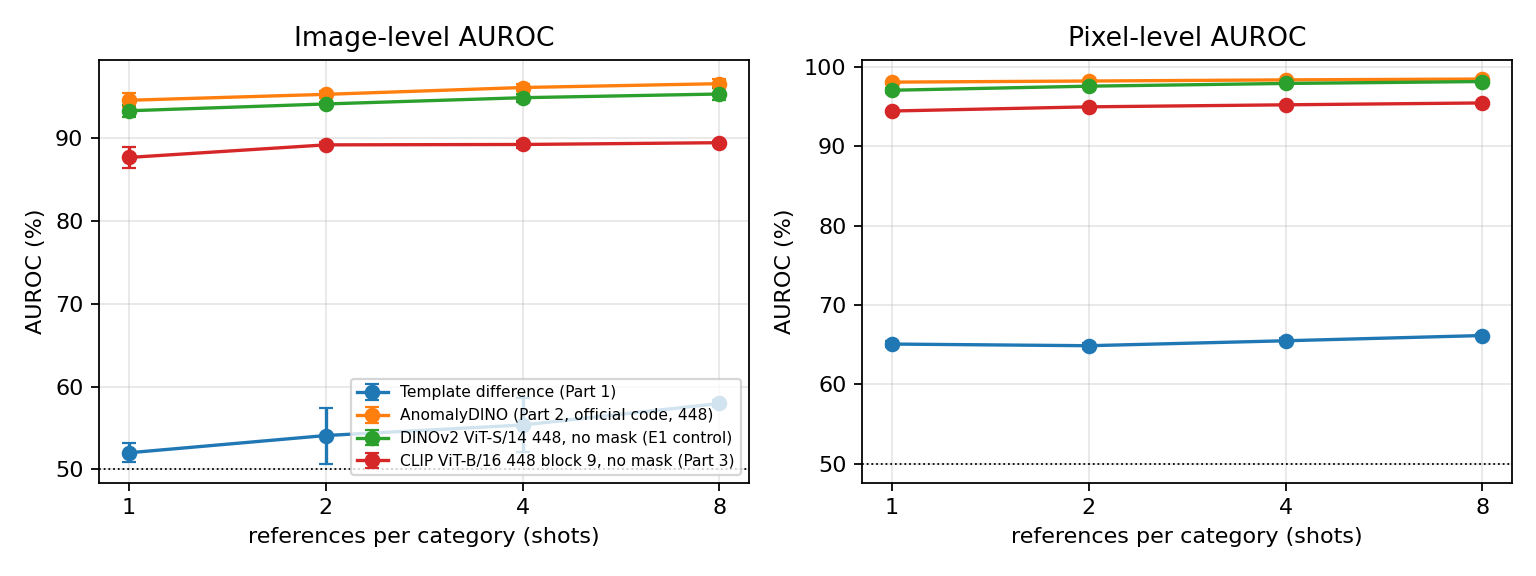
\includegraphics[width=\columnwidth]{figures/auroc_vs_shots.png}
  \caption{Image and pixel AUROC vs number of references, all four systems. The CLIP--DINOv2
  gap is essentially constant in $K$.}
  \label{fig:shots}
\end{figure}

\begin{figure}[t]
  \centering
  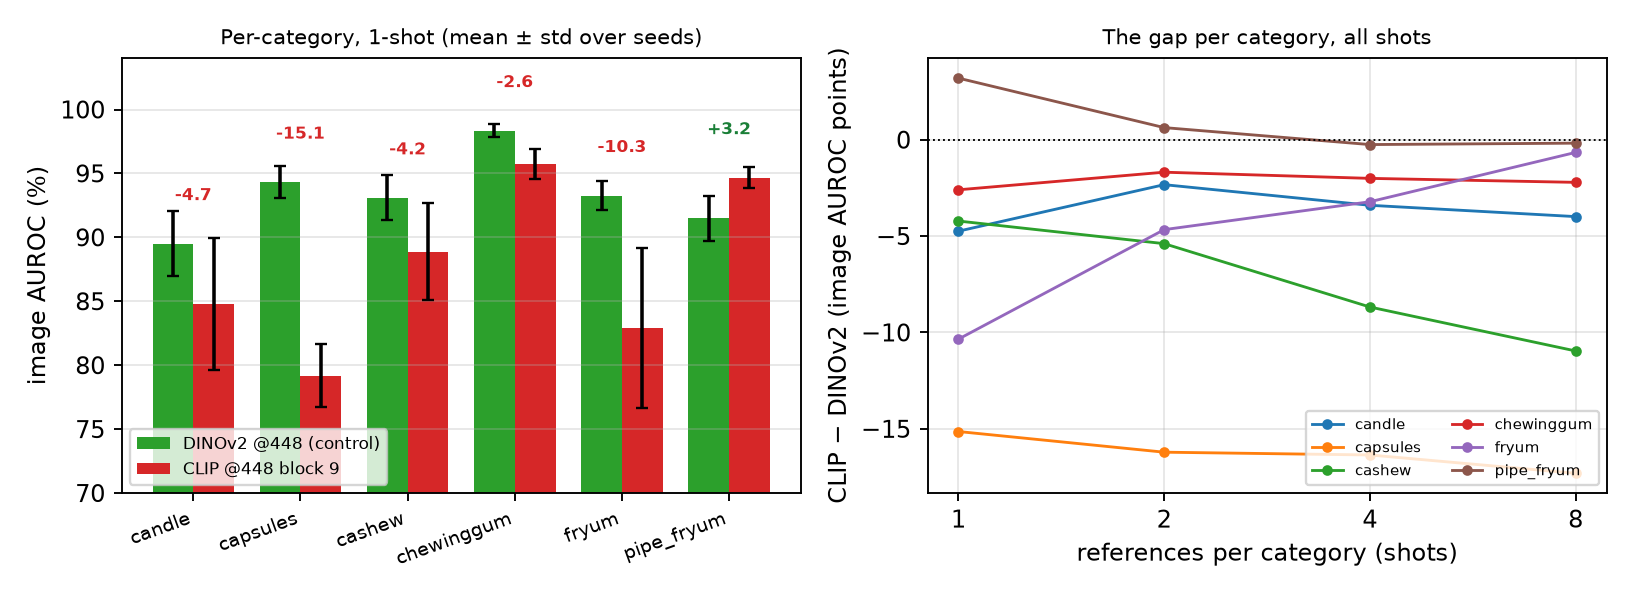
\includegraphics[width=\columnwidth]{figures/per_category_1shot.png}
  \caption{Per-category analysis. Left: 1-shot image AUROC per category (bars, seed std) with
  the CLIP$-$DINOv2 gap annotated. Right: the gap across shot counts. capsules diverges
  ($-15.1 \rightarrow -17.3$), fryum converges ($-10.3 \rightarrow -0.7$), pipe\_fryum is
  reversed ($+3.2$ at 1-shot).}
  \label{fig:percat}
\end{figure}

\subsection{Per-category analysis}
\label{sec:exp-percat}

\begin{table}[t]
\centering
\caption{Per-category gap $\Delta =$ CLIP $-$ DINOv2, image AUROC points (mean over seeds).}
\label{tab:gap}
\small
\begin{tabular}{lrrrr}
\toprule
category & 1-shot & 2-shot & 4-shot & 8-shot \\
\midrule
candle & $-4.7$ & $-2.3$ & $-3.4$ & $-4.0$ \\
capsules & $-15.1$ & $-16.2$ & $-16.4$ & $-17.3$ \\
cashew & $-4.2$ & $-5.4$ & $-8.7$ & $-11.0$ \\
chewinggum & $-2.6$ & $-1.7$ & $-2.0$ & $-2.2$ \\
fryum & $-10.3$ & $-4.7$ & $-3.2$ & $-0.7$ \\
pipe\_fryum & \best{$+3.2$} & $+0.6$ & $-0.3$ & $-0.2$ \\
\bottomrule
\end{tabular}
\end{table}

Three regimes are visible (Table~\ref{tab:gap}, Fig.~\ref{fig:percat}).
\emph{Persistent, large deficits} -- capsules starts 15.1 behind and \emph{widens} to 17.3;
its defects are sub-patch-scale colour/end-cap anomalies where CLIP's 16-px,
language-aligned tokens keep firing on normal background variation (\S\ref{sec:exp-mech}).
\emph{Diverging trends} -- fryum starts 10.3 behind but converges to $-0.7$ at 8-shot, the
only category where more references nearly close the gap. \emph{A reversal} -- pipe\_fryum is
the one category where CLIP is ahead at 1-shot ($+3.2$) and statistically tied at 4/8-shot:
on highly regular, near-periodic objects the globally aligned features are not strictly
worse. An aggregate-only table would hide all three; the reversal and the fryum pixel tie
(CLIP matches the control's pixel AUROC there while trailing 10.3 on image AUROC) are the
quantitative footing for the complementarity claim that the fusion experiments test.

\subsection{Why CLIP trails: anisotropy and map variance}
\label{sec:exp-mech}

The mechanism was measured, not assumed. Patch features inside one image are far more
anisotropic in CLIP's last block -- mean pairwise cosine similarity 0.57--0.67 against 0.36
for DINOv2 L12 -- so nearest-neighbour \emph{distances} compress unevenly across the image.
The layer sweep found block 9 the least anisotropic of \{6, 9, 12\} and the best under the
frozen framing. The direct visual consequence is in Fig.~\ref{fig:heatmaps}: DINOv2's
distance field is near-flat over the background with isolated hotspots, while CLIP's block-9
map is high-variance everywhere, so large areas of \emph{normal} background sit close to the
decision threshold (candle: CLIP's calibration threshold 0.355 vs DINOv2's 0.269 at the same
nominal operating point). Small defects then drown in background variance -- exactly the
capsules ($-15.1$) and fryum ($-10.3$) regime.

\begin{figure}[t]
  \centering
  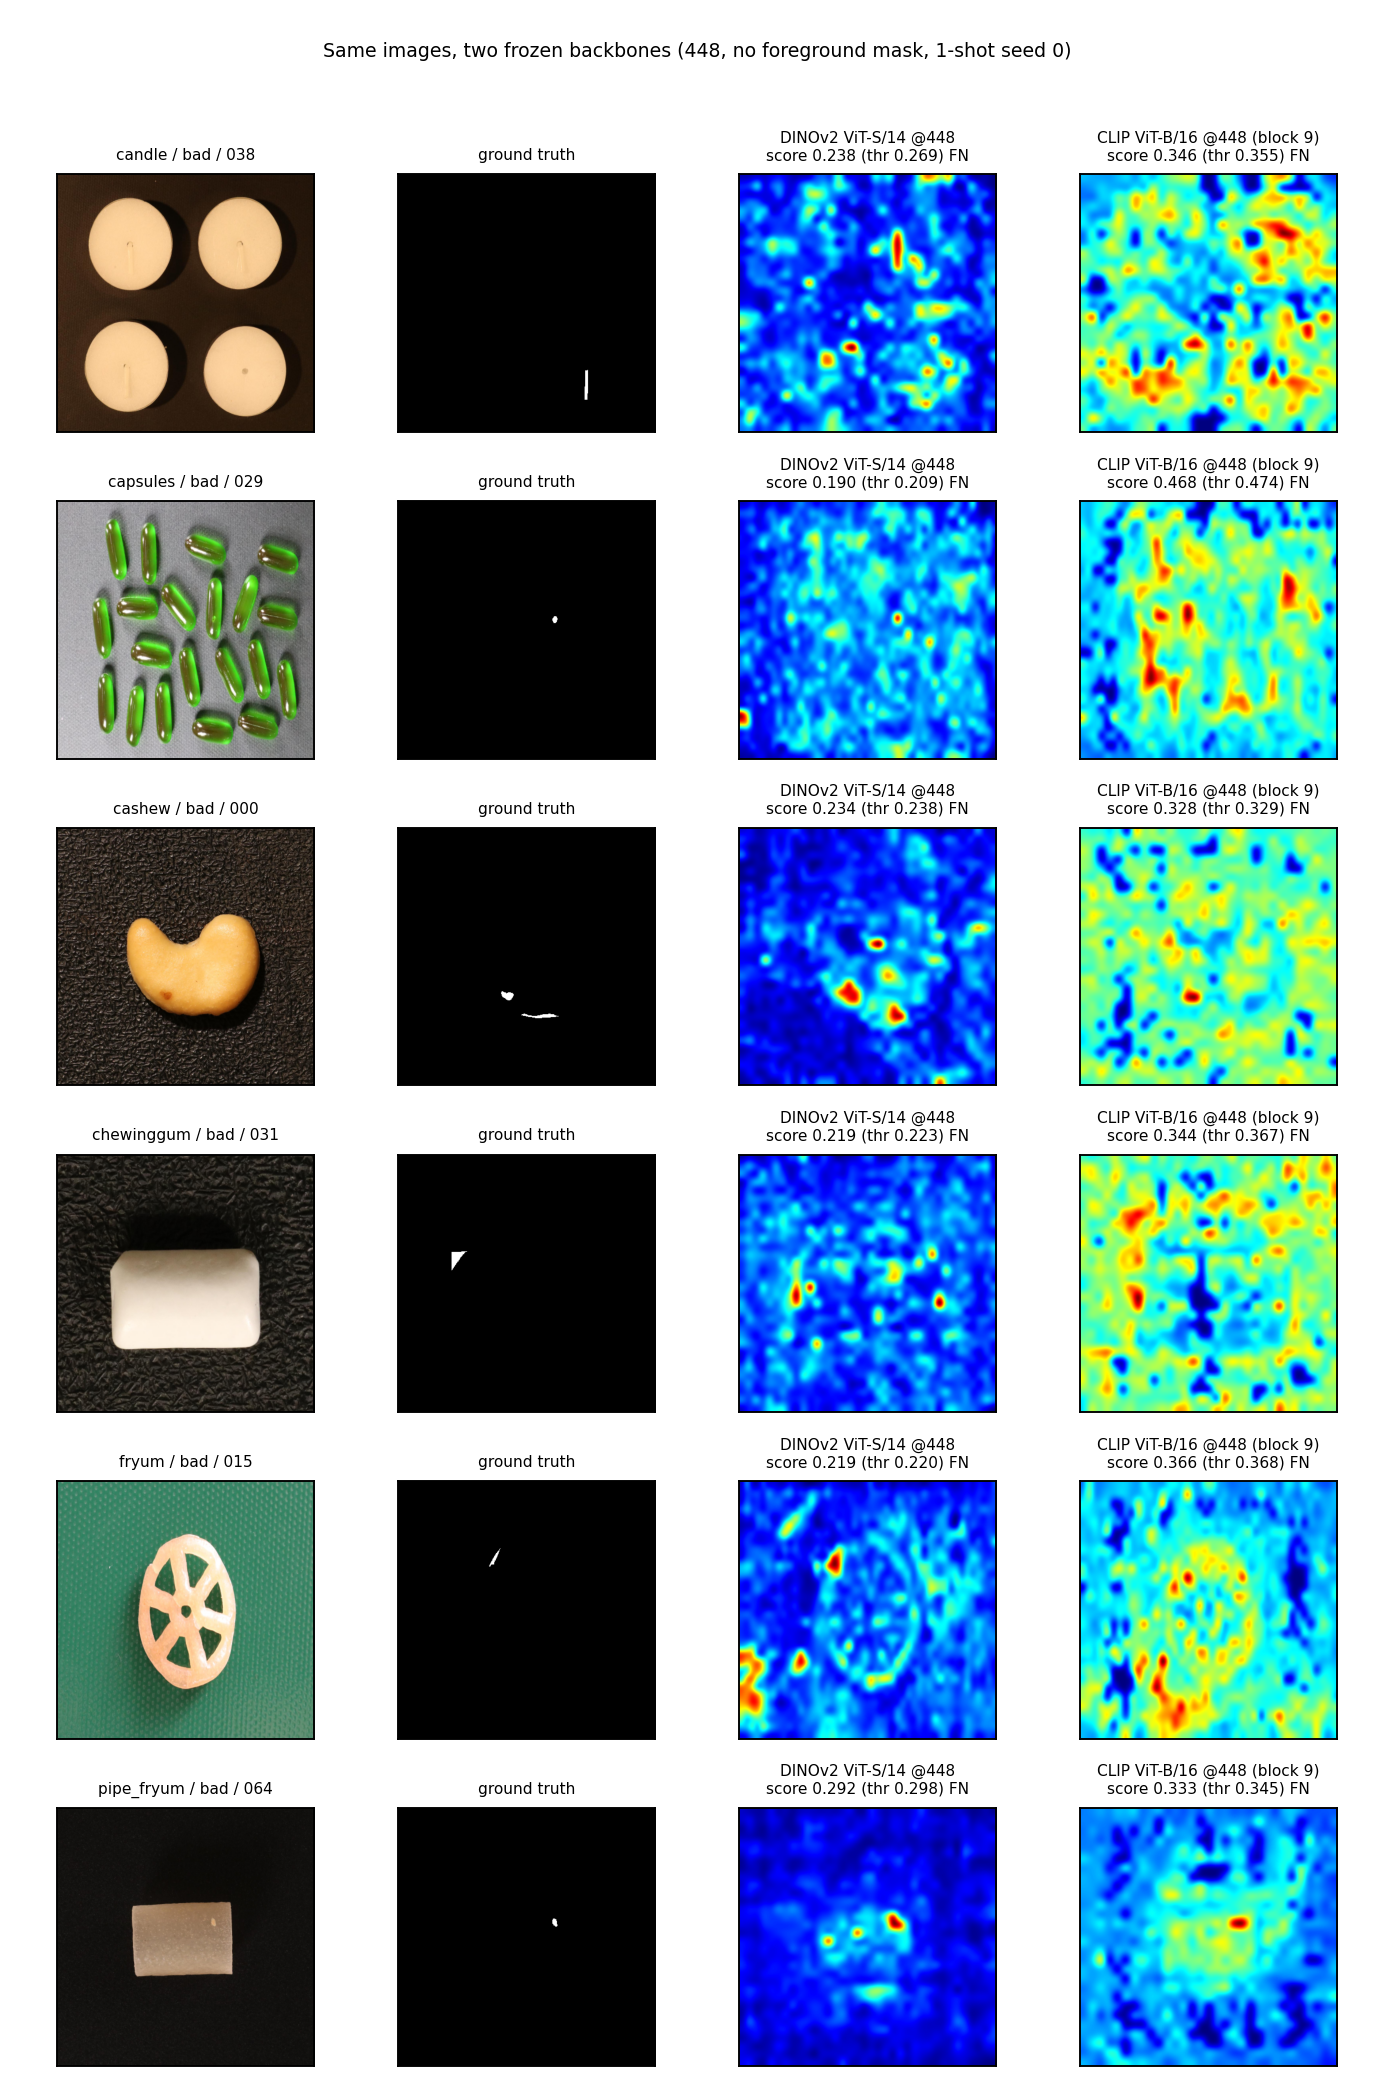
\includegraphics[width=0.94\columnwidth]{figures/heatmap_panel.png}
  \caption{Both-miss cases picked by a fixed rule before either map was inspected: ground
  truth (top), DINOv2 distance map (middle), CLIP block-9 map (bottom) for one image per
  category. DINOv2's field is flat with isolated hotspots; CLIP's is high-variance
  everywhere.}
  \label{fig:heatmaps}
\end{figure}

\subsection{Error taxonomy (1-shot, seed 0)}
\label{sec:exp-taxonomy}

Each test image receives a verdict from its own arm's calibration threshold; the two verdicts
are crossed image-by-image over all 960 test images
(Table~\ref{tab:taxonomy}).

\begin{table}[t]
\centering
\caption{Verdict crossing at each arm's own calibration threshold, 1-shot seed 0 (960 test
images). The fourth cell completes once the multimodal branch's per-image verdicts are in.}
\label{tab:taxonomy}
\footnotesize
\begin{tabular}{lrr}
\toprule
verdict cell & images & share \\
\midrule
both arms right & 607 & 63.2\% \\
only DINOv2 right & 193 & 20.1\% \\
only CLIP right & 58 & 6.0\% \\
both wrong & 102 & 10.6\% \\
\bottomrule
\end{tabular}
\end{table}

The arms agree on only 63.2\% of images. Defects missed by both: 90 of 600; normals flagged
by both: 12 of 360. CLIP is right on \textbf{58 images where DINOv2 is wrong} (35 of them on
candle and pipe\_fryum, the two categories where its deficit is smallest or reversed) -- a
concrete, countable complementarity that bounds any score-fusion gain from below and
motivates \S\ref{sec:exp-fusion}. \bsec{The fourth cell, ``only the VLM is right'', fills
from E2's per-image verdicts.}

\subsection{Score-level fusion of the visual pair -- machinery pilot}
\label{sec:exp-fusion}

\begin{table}[t]
\centering
\caption{Fusion machinery pilot (1-shot, seed 0; \emph{not} comparable with the three-seed
rows of Table~\ref{tab:image}). Fused $=\alpha z_{\mathrm{DINOv2}} + (1-\alpha)
z_{\mathrm{CLIP}}$ after per-category median/MAD standardisation on the 20 calibration
scores. $\alpha{=}1$/$\alpha{=}0$ reproduce the single branches exactly (max deviation 0.0).}
\label{tab:fusion}
\small
\begin{tabular}{lrrrrr}
\toprule
$\alpha$ (weight on DINOv2 $z$) & 0.00 & 0.25 & 0.50 & 0.75 & 1.00 \\
\midrule
image AUROC, macro (\%) & 85.97 & 91.61 & \best{93.75} & 94.05 & 93.11 \\
realised FPR at nominal 5\% & 14.2\% & 16.9\% & 17.5\% & 13.9\% & 9.4\% \\
\bottomrule
\end{tabular}
\end{table}

This subsection validates the fusion protocol before the multimodal branch lands; it must
not be read as a main result. With the pre-registered rule of \S\ref{sec:method-fusion}, the
fused scores on the 960 images of the 1-shot seed-0 cell give Table~\ref{tab:fusion} and
Fig.~\ref{fig:alpha}.

Two honest readings. \emph{Ranking}: at the pre-registered $\alpha = 0.5$ the fused score
beats the better single arm by $+0.64$ points (94.05 at $\alpha = 0.75$ is the sweep's
maximum and is reported as sensitivity only); the gain is bounded by the 58 ``only CLIP
right'' images and is consistent with the taxonomy. \emph{Reliability}: the realised
false-alarm rate at the nominal 5\% threshold is 9.4--17.5\% across $\alpha$, \emph{including
the single branches} -- 20 training-normal calibration images do not cover the variation of
the normal test images, so thresholds must be reported as achieved operating points, not
calibrated guarantees~\cite{guo2017calibration,geifman2017selective}.
\bsec{E3/E4 (DINOv2+Qwen, CLIP+Qwen) and E5 (cross-backbone fusion) upgrade this subsection
to a main result.}

\begin{figure}[t]
  \centering
  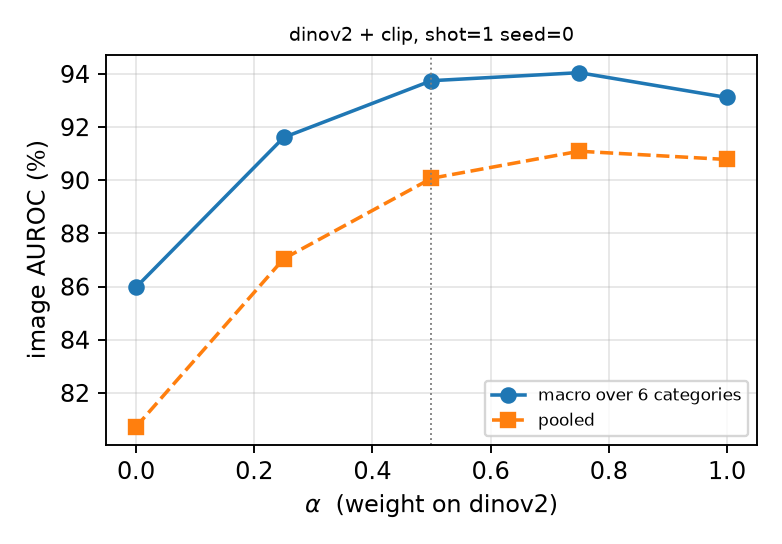
\includegraphics[width=0.94\columnwidth]{figures/fusion_visual_pair_1shot_seed0_alpha.png}
  \caption{Fusion sensitivity: image AUROC and realised false-alarm rate vs $\alpha$, visual
  pair, 1-shot seed 0. The pre-registered $\alpha=0.5$ is marked; the sweep maximum at
  $\alpha=0.75$ is reported as sensitivity only.}
  \label{fig:alpha}
\end{figure}

\subsection{Cost}
\label{sec:exp-cost}

Features are extracted exactly once per backbone and cached in float32; every (shot, seed)
cell afterwards is a $k$-NN pass, and the $\alpha$ sweep after that is offline and costs
milliseconds. Grid wall-clock on the shared RTX A6000 (with the $k$-NN search CPU-bound and
the GPU mostly idle): CLIP grid 265.6\,min, DINOv2 control ${\approx}4$\,h, stage-4 artefacts
(per-image dumps, heatmaps, taxonomy, tables, curves) ${\approx}27$\,min.

Per-image inference cost is measured separately at batch size 1
(Table~\ref{tab:cost}): end-to-end latency of one test image -- decode, resize/normalise,
upload, backbone forward, 1-NN over the reference bank, top-1\% pooling and the pixel-map
resize -- with feature extraction \emph{included} and the one-off reference-bank construction
amortised, plus peak CUDA memory on the same device.

\begin{table}[t]
\centering
\caption{Measured per-image inference cost (batch size 1, RTX A6000, faiss/BLAS threads
pinned to 1). Feature extraction included; reference-bank construction amortised; peak memory
from the CUDA allocator. \tbd{a}: paste from \texttt{scripts/bench\_inference.py};
\tbd{b}: measured by the multimodal branch's owner.}
\label{tab:cost}
\footnotesize
\setlength{\tabcolsep}{3.0pt}
\begin{tabular}{lrrr}
\toprule
Encoder & Lat.\ (ms) & Mem (MiB) & Par.\ (M) \\
\midrule
DINOv2 ViT-S/14 @448 & \tbd{a} & \tbd{a} & 22.1 \\
CLIP ViT-B/16 @448 L9 & \tbd{a} & \tbd{a} & 86.2 \\
Qwen-VL branch (E2) & \tbd{b} & \tbd{b} & \tbd{b} \\
\bottomrule
\end{tabular}
\end{table}

\subsection{Threats to validity}
\label{sec:exp-threats}

The controlled arms differ in patch size (14 vs 16\,px) and parameter count (22\,M vs 86\,M
vision parameters), so E1 measures \emph{this} CLIP encoder against \emph{this} DINOv2
encoder, not ``CLIP vs DINOv2'' in general; no patch-size-matched pair is publicly released.
CLIP runs at a resolution and normalisation different from its pretraining setup; the bicubic
position-table interpolation addresses this and is probe-verified but cannot be perfect. The
fusion pilot is one cell (1-shot, seed 0) of the two \emph{visual} arms; nothing in it may be
generalised until the per-(shot, seed) grid and the multimodal branch are in. Finally, all
six categories are object-centric product photographs; none of these conclusions should be
quoted for texture categories or scene-level anomalies, and MVTec AD~2's harder
scenarios~\cite{hecklerkram2026mvtec2} indicate the easier part of the problem space is what
we measure.

\section{Conclusion}
\label{sec:conclusion}

We asked how far a frozen encoder carries few-shot industrial anomaly detection. A verified
AnomalyDINO reproduction anchors the visual route at 94.61 image AUROC on VisA's six
object-centric categories at 1-shot; a controlled encoder swap shows CLIP's vision tower
gives up 5.6 points in dense patch matching -- a property of the features, not of sample
size; the arms disagree on 36.8\% of images, leaving room for the pre-registered fusion to
gain $+0.68$ points across nine (shot, seed) cells, at calibration gaps reported as achieved
operating points, not guarantees.

In practical terms the trade-off is explicit. When latency or memory dominates, DINOv2 alone
is the operating point (148.5\,ms, 120\,MiB per image), and the confirmed DINOv2--CLIP fusion
gains $+0.68$ points and lowers the cross-cell spread. Qwen2-VL-7B has the highest
ranking point estimate on the matched holdout, but its advantage over DINOv2 is uncertain
across reference seeds. Its scoring stage alone took 2.64\,s per image with 23.47\,GB
mean peak allocation in a separate run; it produces no pixel heatmap.

\textbf{Limitations.} All six categories are object-centric product photographs, so nothing
here speaks to texture or scene-level anomalies, and MVTec~AD~2's harder
scenarios~\cite{hecklerkram2026mvtec2} mark where our conclusions stop. The Qwen branch was
scored on 696 images reused across three reference sets, so the seed comparison tests reference stability on the same images, and its threshold recall (25.6\% on cashew) is too weak to
drive an OK/NG decision alone. Latency and memory come from a shared GPU with a second
tenant active.

\textbf{Future work.} Extend the protocol to MVTec~AD~2's lighting and contamination
scenarios and to texture categories; confirm or reject the Qwen--DINOv2 fusion on a fresh
held-out split instead of the post-hoc 97.68; replace the 20-image percentile threshold with
a calibration set large enough to hold the nominal false-alarm rate; and test whether a
foreground mask transferred from a general segmenter recovers the 1.3 points it is worth
without re-introducing the backbone as a second variable.

The wider lesson is methodological: with no training signal, every claim reduces to the
representation or the decision rule, so both are measured under a protocol frozen before
scoring, with per-image evidence for every aggregate and reliability next to accuracy.


{\small
\bibliographystyle{ieeenat_fullname}
\bibliography{references}
}

% ---------------- reproducibility appendix (kept inside the page budget check)
\clearpage
\appendix
\onecolumn
\section*{Reproducibility appendix}
\label{app:repro}

\paragraph{Repository.}
Everything in this report is generated from
\url{github.com/BEBE2777/computer-vision-aiaa3201}. The mapping from claim to artefact:

\begin{table}[h]
\centering
\small
\begin{tabular}{p{0.30\columnwidth}p{0.58\columnwidth}}
\toprule
Report element & Artefact in the repository \\
\midrule
Part 1 grid & \texttt{results/tables/} (template-difference runner) \\
Part 2 official numbers & \texttt{results/part2\_official/}, parity report \texttt{parity\_report.md} \\
Part 2 cached authority & \texttt{results/part2\_cached/base\_L12\_v2\_final.json} \\
E1 grids & \texttt{results/part3/tables.md}, \texttt{e1\_full.md}, \texttt{metrics.json} \\
Per-image dumps & \texttt{results/part3/scores/*.json} (960 images per arm) \\
Error taxonomy & \texttt{results/part3/error\_cases.csv}, \texttt{error\_taxonomy.md};
3-way with Qwen: \texttt{error\_taxonomy\_qwen\_696.md} \\
Multimodal branch (E2) & \texttt{results/extensions/qwen/}: frozen protocol
\texttt{PROTOCOL\_FROZEN.md}, v4 confirmation \texttt{confirm\_full\_v4/REPORT\_V4.md},
per-image scores \texttt{predictions\_v4\_test.json}, reference-seed stability
\texttt{stability\_v5/REPORT\_V5.md} \\
Fusion & \texttt{results/part3/fusion/dinov2\_clip\_9cells.md}, scripts \texttt{scripts/score\_fusion.py}, \texttt{scripts/fuse\_sweep.py} \\
Figures & \texttt{scripts/plot\_per\_category.py}, \texttt{scripts/plot\_pipeline.py}, \texttt{make\_figures.py}, \texttt{scripts/make\_heatmap\_panel.py} \\
Latency / memory & \texttt{scripts/bench\_inference.py}, \texttt{scripts/run\_bench.sh} \\
Protocol freezes & \texttt{docs/part3/} (planning, method and experiments drafts) \\
\bottomrule
\end{tabular}
\end{table}

\paragraph{Environment.}
Shared NVIDIA RTX A6000 (48\,GB), one GPU job at a time; PyTorch with CUDA; faiss
\texttt{IndexFlatL2} with \texttt{OMP\_NUM\_THREADS=1} (small $k$-NN searches are
synchronisation-bound); all cached features float32; feature cache on persistent disk,
large scratch files under \texttt{/tmp}.

\paragraph{Determinism.}
Reference pools are sorted and sliced deterministically
($\text{pool}[s\,\text{shot}:(s{+}1)\,\text{shot}]$); the PCA foreground mask uses a pinned
random state (a randomized-PCA seed flip otherwise moved up to 460 of 1024 patches on one
category); augmentation is a fixed set of 8 rotations; no test label enters thresholding,
weight selection or any other choice.

\paragraph{Data.}
VisA~\cite{zou2022spot} official \texttt{1cls} split, six object-centric categories, 960 test
images in total. No dataset images, model weights or large caches are committed to the
repository; the README documents how to fetch them.


\end{document}
